%!TEX root = ../thesis.tex

\section{背景}
近年, 様々なセンサを用いた自律移動に関する研究が活発に行われており, その中で視覚を入力としたend-to-end学習により自律走行した例もある. 例えば, Bojaskiらは\figref{Fig:bojaski}に示すシステムでカメラ画像と人が操作するステアリングの角度をend-to-end学習することで, 自律走行する手法を提案した\cite{bojaski}.

\vspace{20mm}

\begin{figure}[hbtp]
\centering
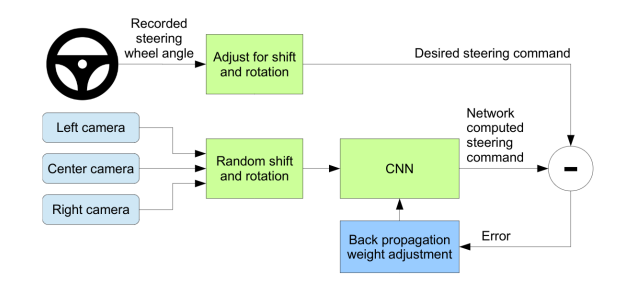
\includegraphics[keepaspectratio, scale=0.5]
{images/bojaski.png}
\caption{Training the neural network from \cite{bojaski}}
\label{Fig:bojaski}
\end{figure}

\newpage
岡田らにより\figref{Fig:tsudanuma2-3}のように地図ベースのナビゲーションによる出力を模倣することで, 経路追従行動を獲得した\cite{okada-si}. \figref{Fig:okada-method}に示すような, LiDAR, オドメトリを入力としたナビゲーションの出力をend-to-endで模倣学習し, 学習後はカメラ画像を入力とした学習器の出力により, 一定の経路において周回が可能であることが確認された. 

\vspace{20mm}

\begin{figure}[h]
     \centering
     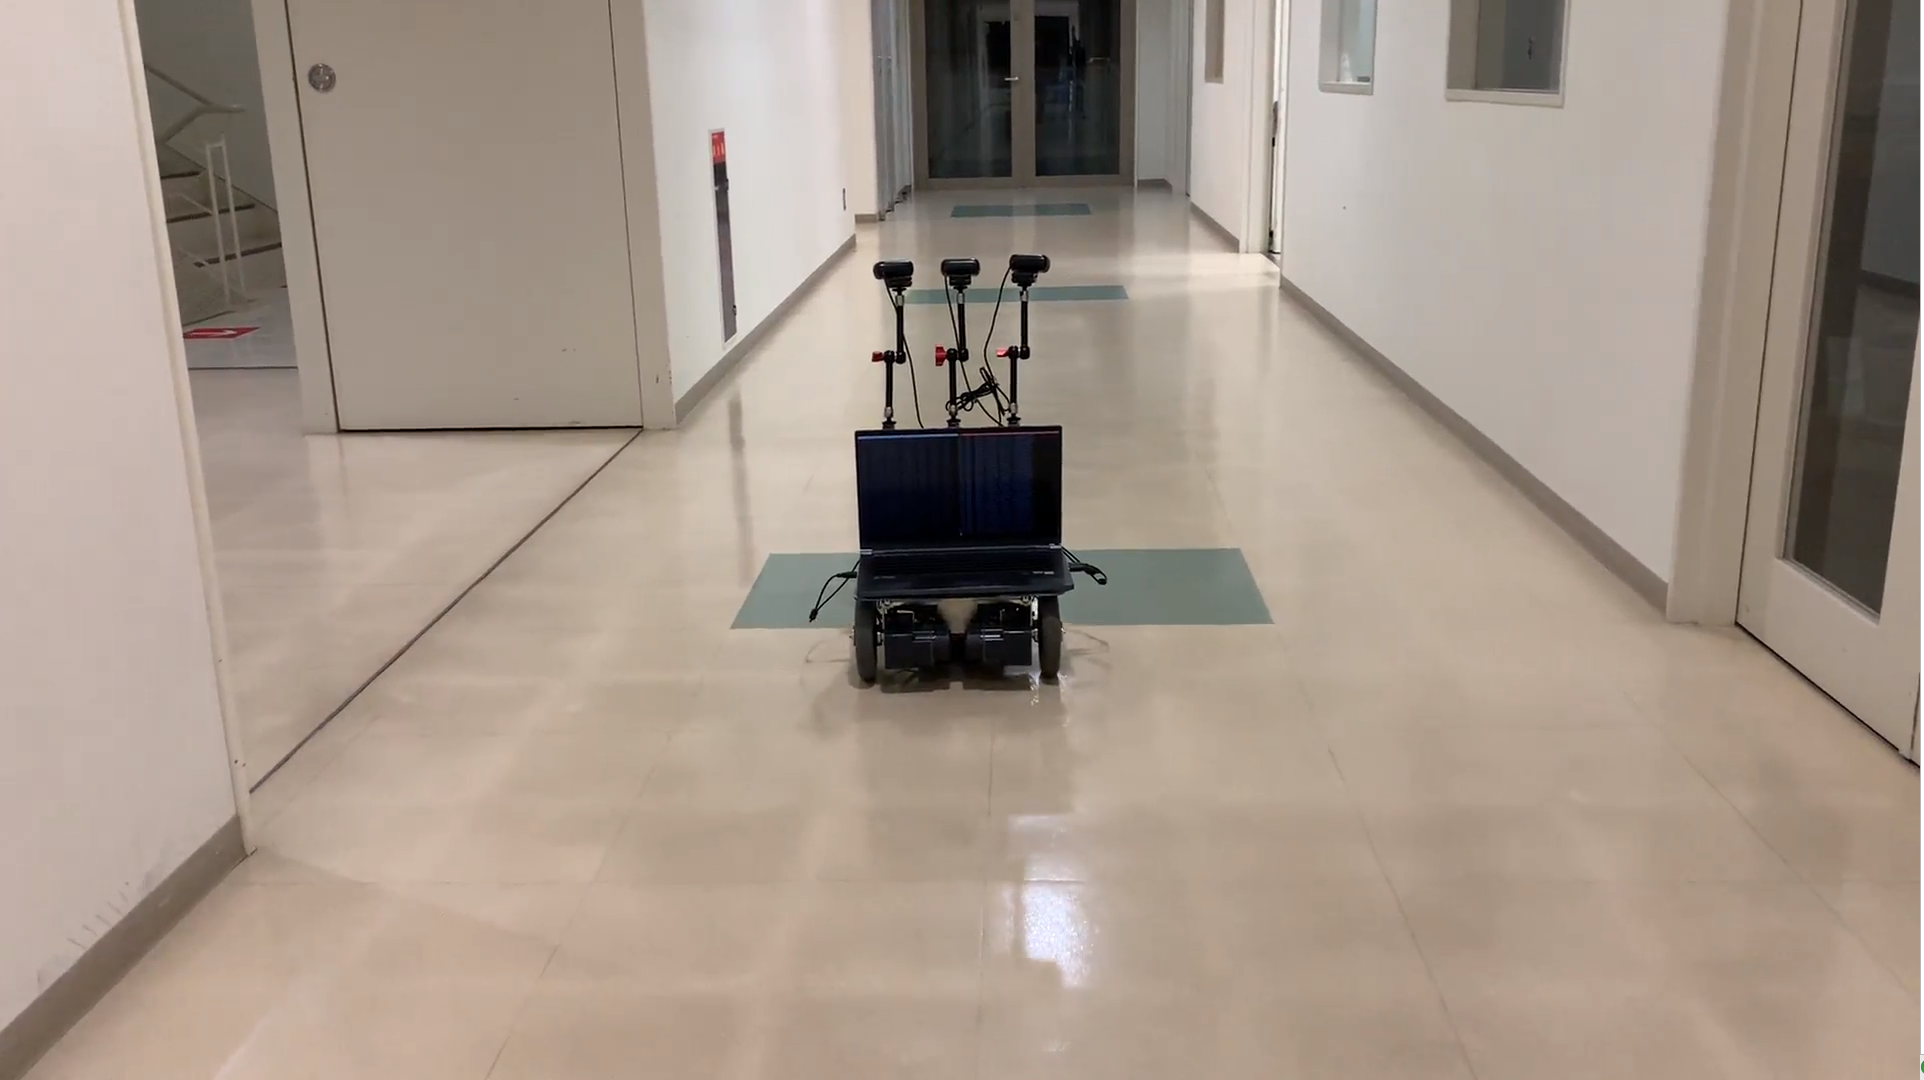
\includegraphics[keepaspectratio, scale=0.15]
     {images/tsudanuma2-3.png}
     \caption{Driving with output from map-based navigation indoors from \cite{okada-si}}
     \label{Fig:tsudanuma2-3}
     \end{figure}

\begin{figure}[h]
     \centering
     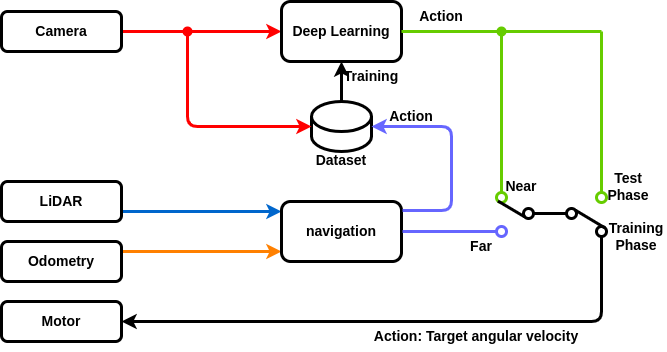
\includegraphics[keepaspectratio, scale=0.45]
     {images/okada-method.png}
     \caption{Okada and others proposed method from \cite{okada-si}}
     \label{Fig:okada-method}
     \end{figure}

\newpage
また, 清岡ら\cite{kiyooka-si}(以下「先行研究」と称する)により, {Fig:kiyooka-si}に示すような手法を用いて, 経路上だけでなく経路から離れた状態も学習することが, 経路追従行動を模倣する上で有効であることが示された. 

\vspace{10mm}

\begin{figure}[h]
     \centering
     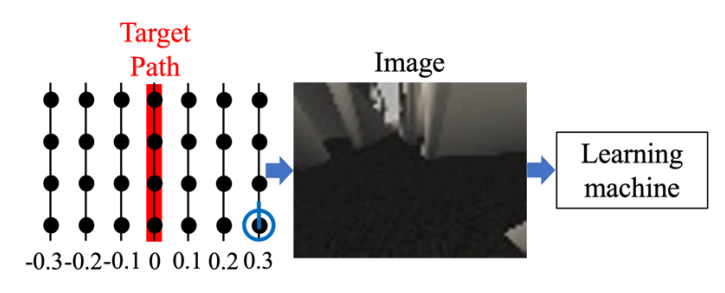
\includegraphics[keepaspectratio, scale=0.45]{images/kiyooka-si-1.png}
     \caption{Kiyooka and others proposed method from \cite{kiyooka-si}}
     \label{Fig:kiyooka-si}
     \end{figure}

\vspace{20mm}
以上で述べたように, カメラ画像を入力とした学習器の出力により, ロボットが学習した経路を周回可能であることが示されている. \par 次に, 先行研究を基に, 新たなデータセットの収集方法を考案する.

\newpage
\section{目的}
本研究では, 先行研究を基に, 新たなデータセットの収集方法を提案する. 提案手法の有効性をシミュレータを用いた実験により検証することを目的とする. 

\section{論文構成}
本論文の構成は以下に述べる通りである. 第1章では, 研究を行う背景や目的を述べた. 
     
